\section{Decomposing Galaxy SEDs} \label{Sec: CIGALE}

We seek to expand upon our investigation of LFs within ZFOURGE by focusing on the contributions of SF regions and AGN within the sample's galaxies. The public version of the ZFOURGE catalogues has utilised \texttt{EAZY} \citep{brammer_eazy_2008} and \texttt{FAST} \citep{kriek_ultra-deep_2009} for parameterising galaxy properties, primarily focusing on photometric redshifts, stellar masses, and SFRs. However, while effective, these methods provide a more generalised view of galaxy properties without entirely disentangling the contributions from different physical components within each galaxy.

To improve upon this, we employ SED fitting using CIGALE, \citep{boquien_cigale_2019} a more sophisticated approach that allows for the decomposition of observed light from galaxies into distinct components, such as SF and AGN activity. This method not only continues to derive critical parameters similar to \texttt{EAZY} and \texttt{FAST} $-$ but it does so with enhanced precision and additional capabilities \citep{boquien_cigale_2019}. Notably, CIGALE allows us to quantify the AGN contribution in each galaxy, which was not addressed previously in ZFOURGE. 

By using this method, we are able to construct more accurate LFs for both SF and AGN components, reducing the bias against low-luminosity AGN that often skews traditional analyses. While our approach builds on the work detailed in \cite{cowley_decoupled_2018}, it includes several key advancements. Specifically, we expand the methodology to incorporate all available photometric bands from the ZFOURGE survey, covering wavelengths from 0.2 $\mu$m to 160 $\mu$m in the CDFS field and up to 24 $\mu$m in COSMOS and UDS. This broader wavelength coverage allows for a more complete and precise decomposition of galaxy light into SF and AGN components.

In addition, we employ an updated parameter space that includes the SKIRTOR AGN torus model \citep{stalevski_dust_2016}, which better accounts for clumpy dust distributions and polar dust extinction. These enhancements, combined with the expanded photometric data, enable us to more effectively quantify AGN contributions and produce more accurate galaxy property estimates. Table \ref{tab:parameter_space} outlines the specific parameters used in this analysis, providing the details of our refined methodology.

\begin{table}[htbp]
\centering
\caption{Parameter space used for SED fitting with CIGALE}
\label{tab:parameter_space}
\begin{tabular}{ll}
\hline
\textbf{Parameter}          & \textbf{Model/Values}                                                           \\ \hline
SFH                         & Delayed SFH $\tau = 1,3,5,7,9,11$ Gyr                                           \\
Age                         & $0.5, 1, 3, 5, 7, 9, 11$ Gyr                                                   \\
Burst Fraction              & $0.0, 0.01, 0.05, 0.1, 0.15, 0.2, 0.3$                                         \\
SSP                         & Bruzual \& Charlot (2003)                                                      \\
IMF                         & Chabrier (2003)                                                             \\
Metallicity                 & Fixed at 0.02                                                                  \\
Nebular                     & Inoue (2011)                                                                   \\
Dust Atten.                 & \cite{calzetti_dust_2000} $E_{(B-V)} = 0.01, 0.05, 0.1, 0.5, 1.0, 1.5$               \\
Dust Emission               & \cite{dale_two-parameter_2014} $\alpha = 1.0, 1.5, 2.0, 2.5, 3.0$                           \\
AGN Model                   & SKIRTOR (Stalevski et al. 2012 \cite{stalevski_dust_2016}                                           \\
Torus Inclination           & $30^\circ, 70^\circ$                                                           \\
AGN Fraction                & $0.0, 0.01, 0.1 - 0.9$ (steps of 0.1), 0.99                                    \\
Polar Extinction            & SMC $E(B-V) = 0.0, 0.03, 0.1, 0.2, 0.4, 0.6, 1.0, 1.8$                   \\
\hline
\end{tabular}
\end{table}

\begin{figure}
    \centering
    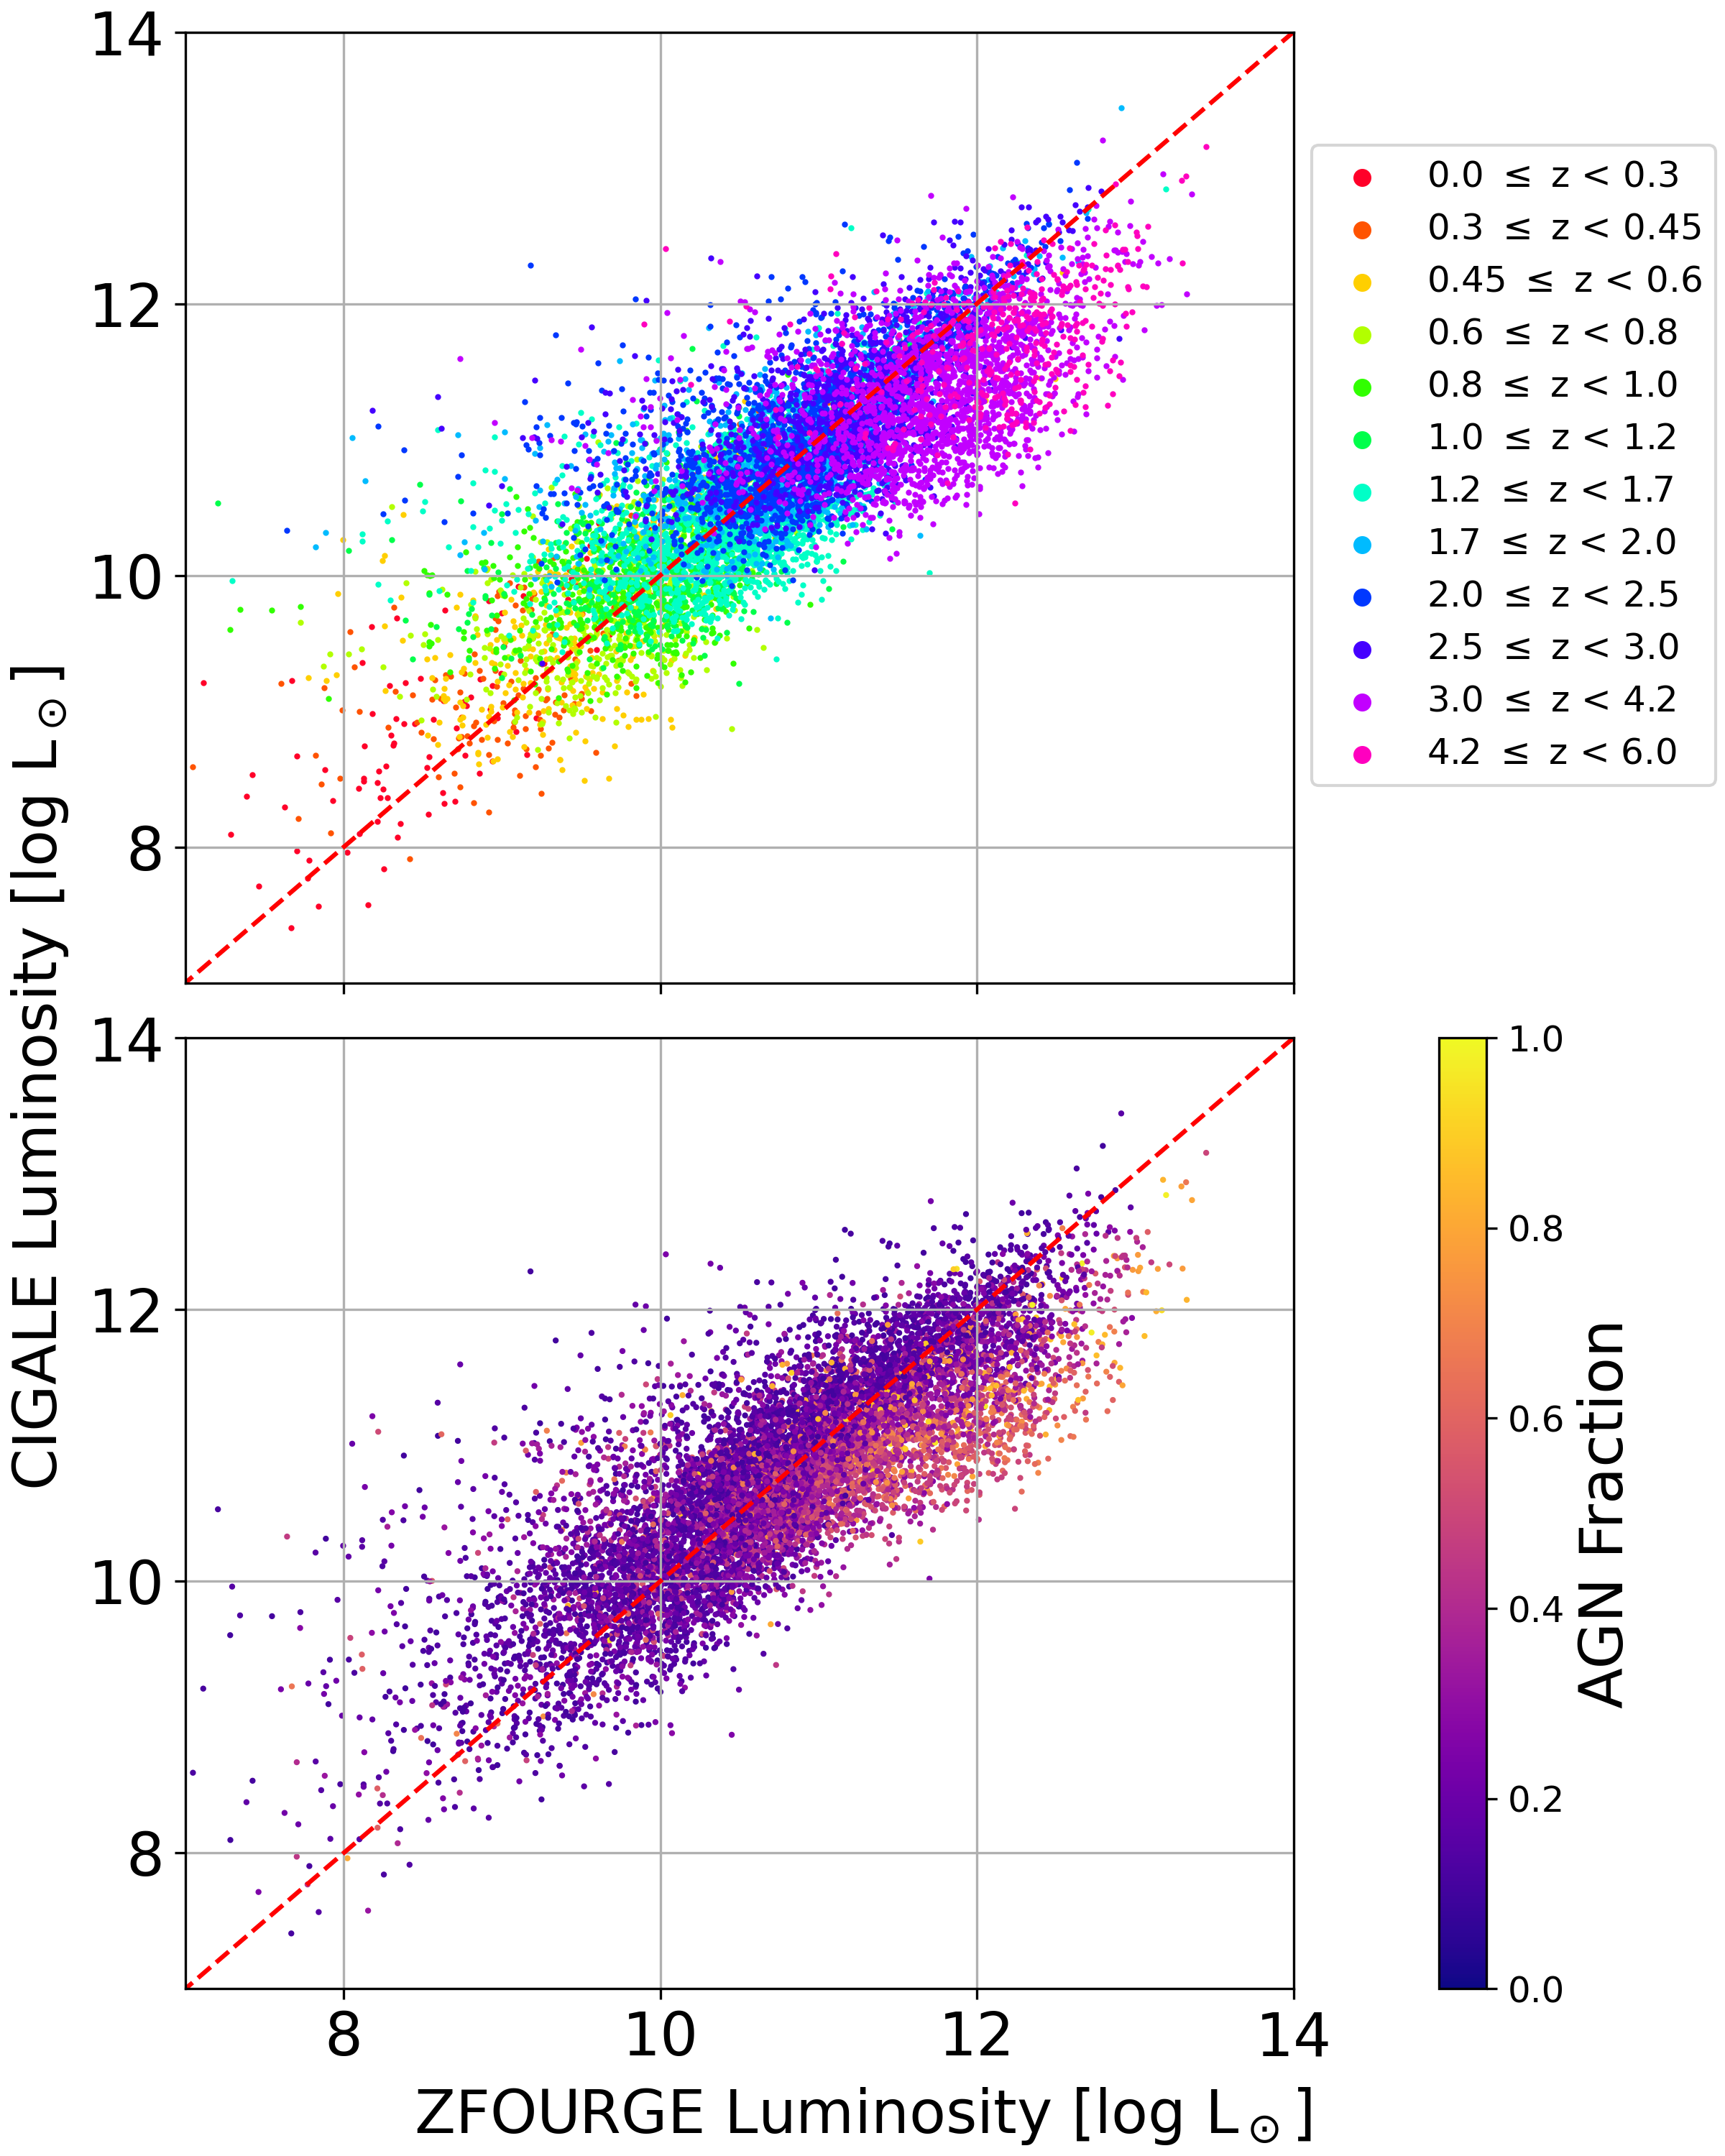
\includegraphics[width=0.48\textwidth]{Figures/LIR vs LIR.png}
    \caption{ZFOURGE bolometric 8-1000$\mu$m IR luminosity compared to CIGALE total luminosity. Top: Sources coloured by redshift bin. Bottom: sources coloured by AGN fraction ($\mathcal{F}_{AGN}$). AGN fraction clearly increases with redshift. At $z \geq 3$ the average AGN fraction is greater than 30\%.}
    \label{Fig: LIR vs LIR}
\end{figure}

\begin{figure*}
    \centering
    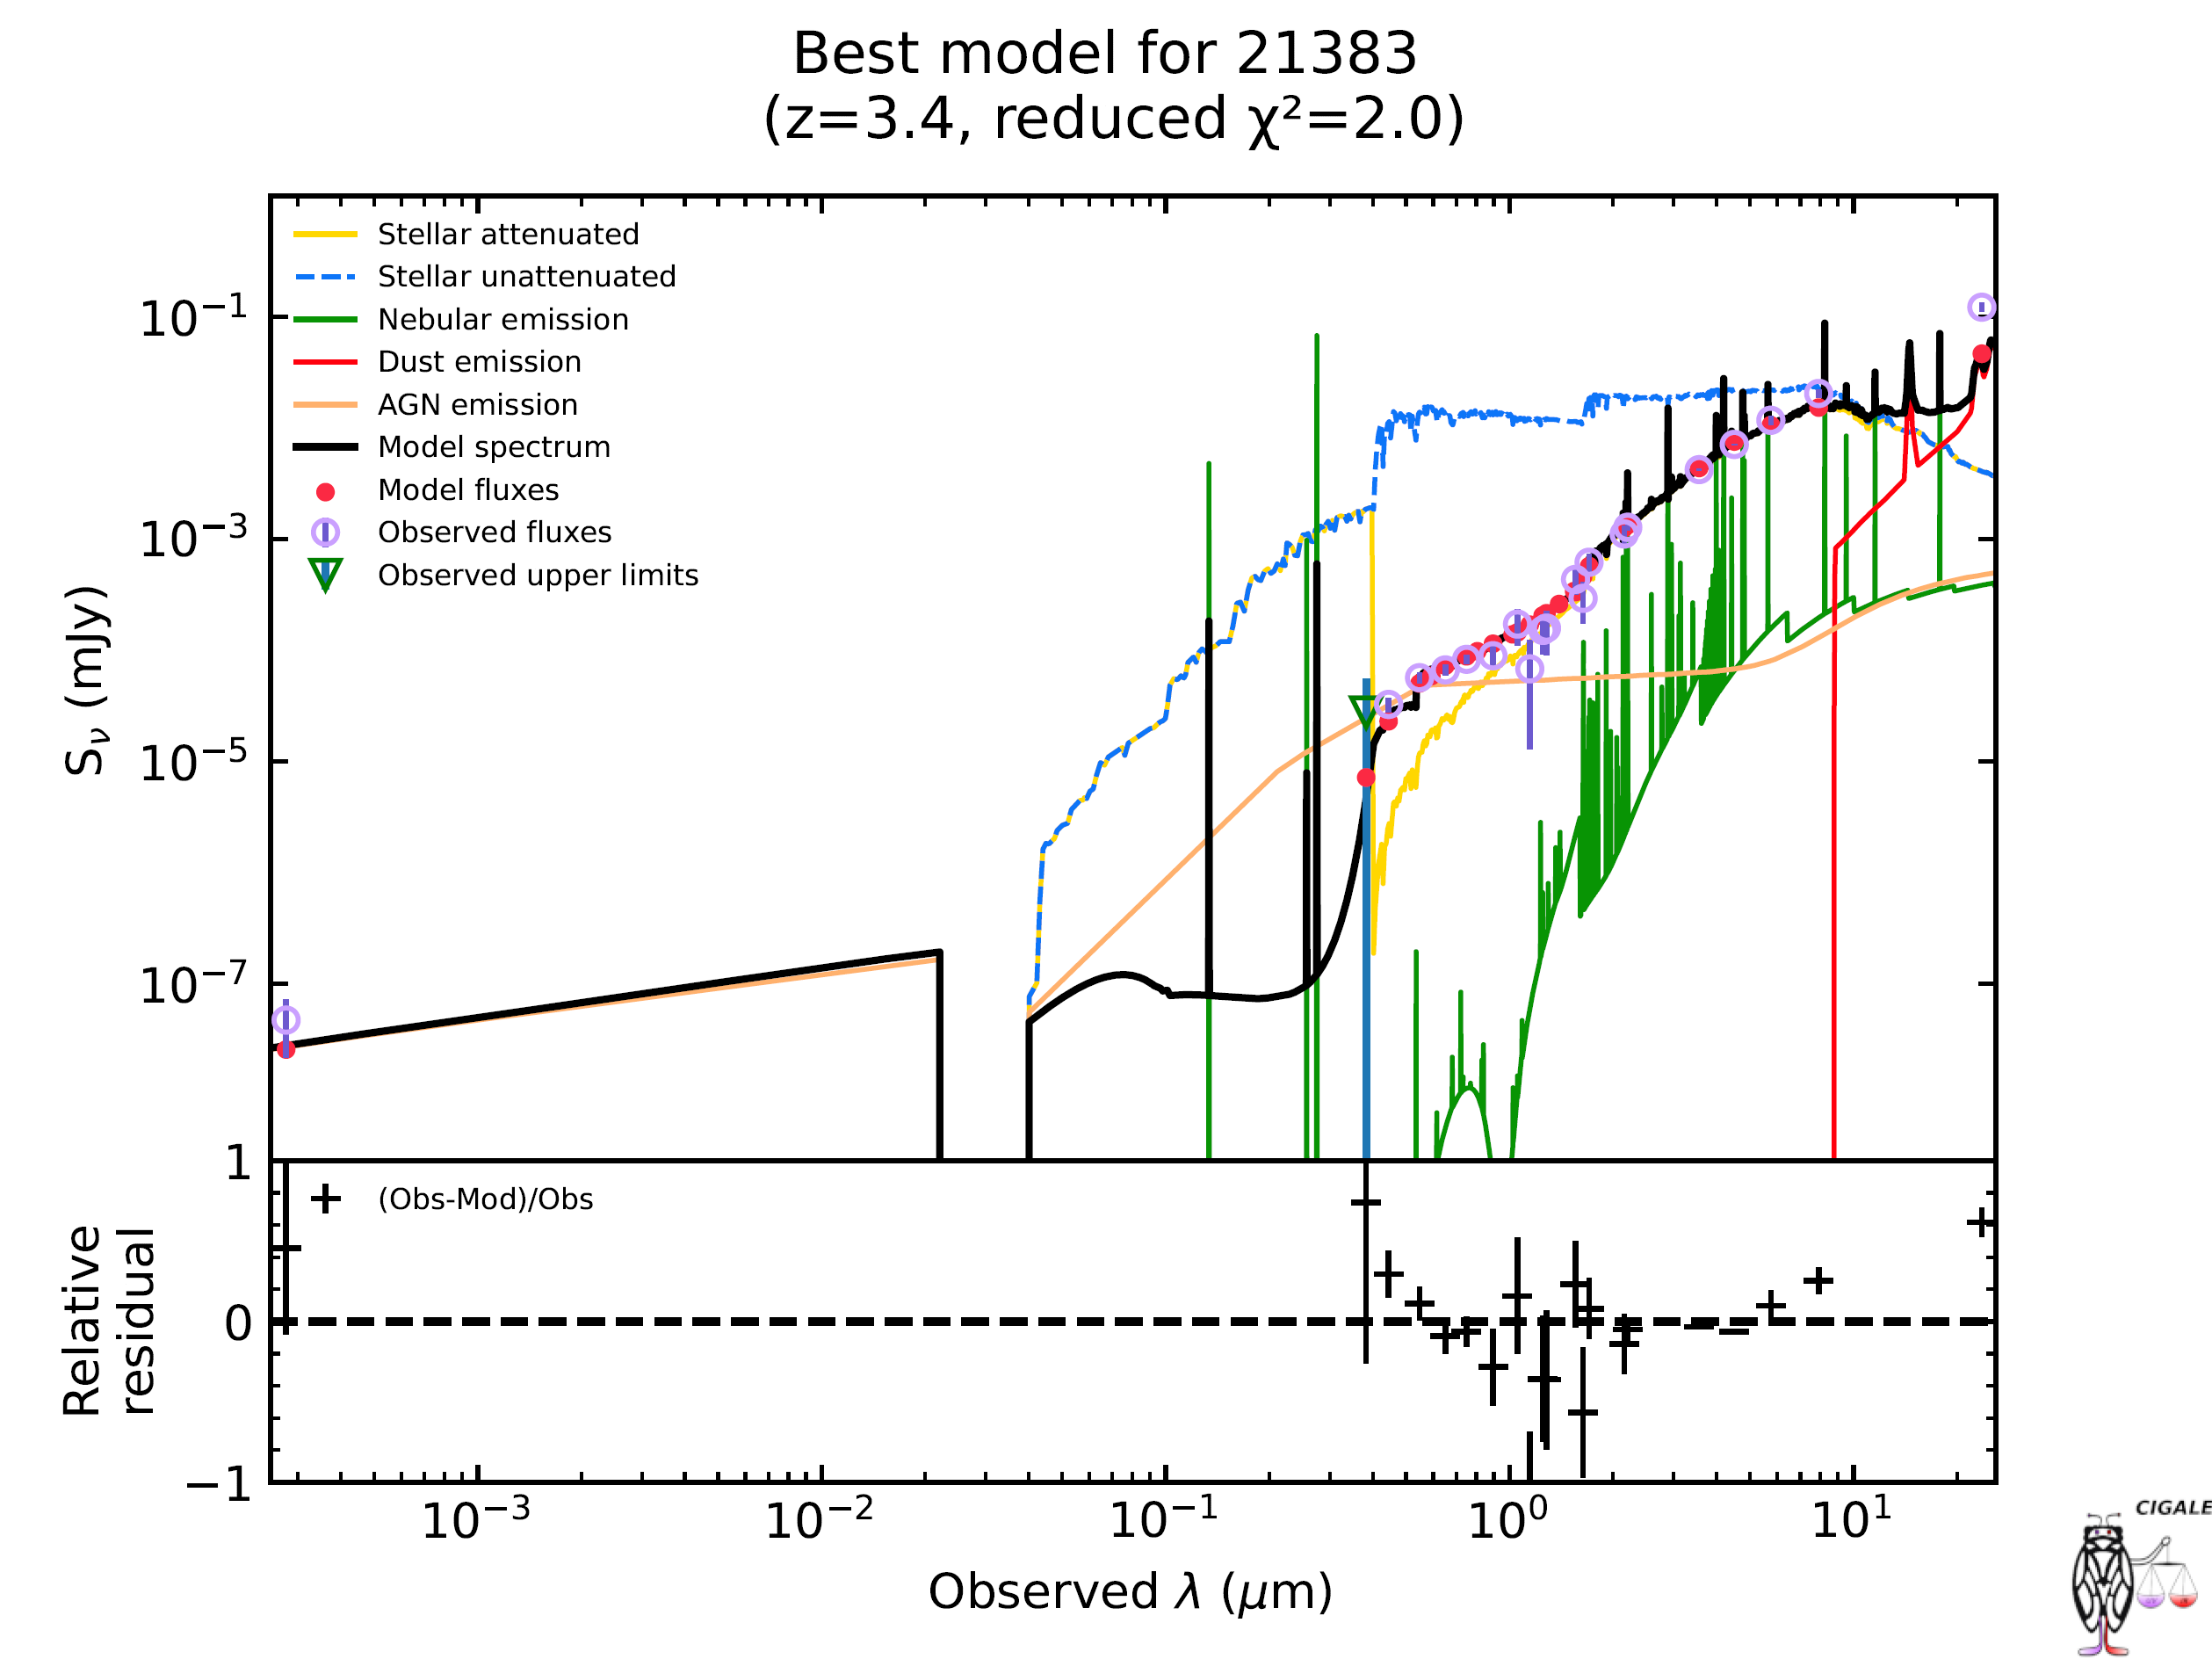
\includegraphics[width=\textwidth]{Figures/SED Example.png}
    \caption{Example SED of different galactic components.}
    \label{Fig: SED Example}
\end{figure*}

To ensure the reliability of AGN extraction, particularly for low-luminosity AGN, we performed a series of robustness tests using mock analysis. These tests evaluated CIGALE's ability to accurately decompose AGN and SF contributions across a range of redshifts and luminosities, with a specific focus on galaxies with low bolometric luminosities. By comparing the input and recovered AGN luminosities from the simulated datasets, we confirmed that our parameter space and methodology are robust, particularly in detecting faint AGN.

The mock analysis demonstrated that AGN luminosity was reliably constrained, with Pearson correlation coefficients (PCCs) ranging from 0.969 to 0.973 across all fields. Most sources lay within 0.5 dex of the 1-to-1 line, with mean residuals between $-0.02$ and $0.04$ dex, confirming the robustness of AGN luminosity recovery. These results indicate that our method effectively minimises bias against low-luminosity AGN, which are often difficult to detect in traditional analyses.

\subsection{Bolometric IR Luminosity Derivation}
\label{sec: Bolometric IR Luminosity}

Understanding the total IR energy output of galaxies is essential for tracing both SF and AGN activity, particularly in dusty environments where much of the energy is re-emitted in the IR \citep{fu_decomposing_2010}. By estimating the bolometric IR luminosity, we can gain insights into the contribution of these processes across cosmic time. To this end, we integrate the best-fit SED of each source from 8-1000$\mu$m to estimate the bolometric IR luminosity, providing a robust measure of the total IR emission. Specifically, we use the averaged \cite{wuyts_fireworks_2008} template to fit the 24-160$\mu$m photometry, from which the total bolometric IR luminosity is derived. For a detailed description of this calculation, refer to section 6 of \cite{straatman_fourstar_2016}. These bolometric IR luminosities are subsequently used to construct the bolometric IR luminosity function of the ZFOURGE survey up to $z \approx 6$ (see section \ref{Sec: Luminosity Functions}).

\begin{figure}
    \centering
    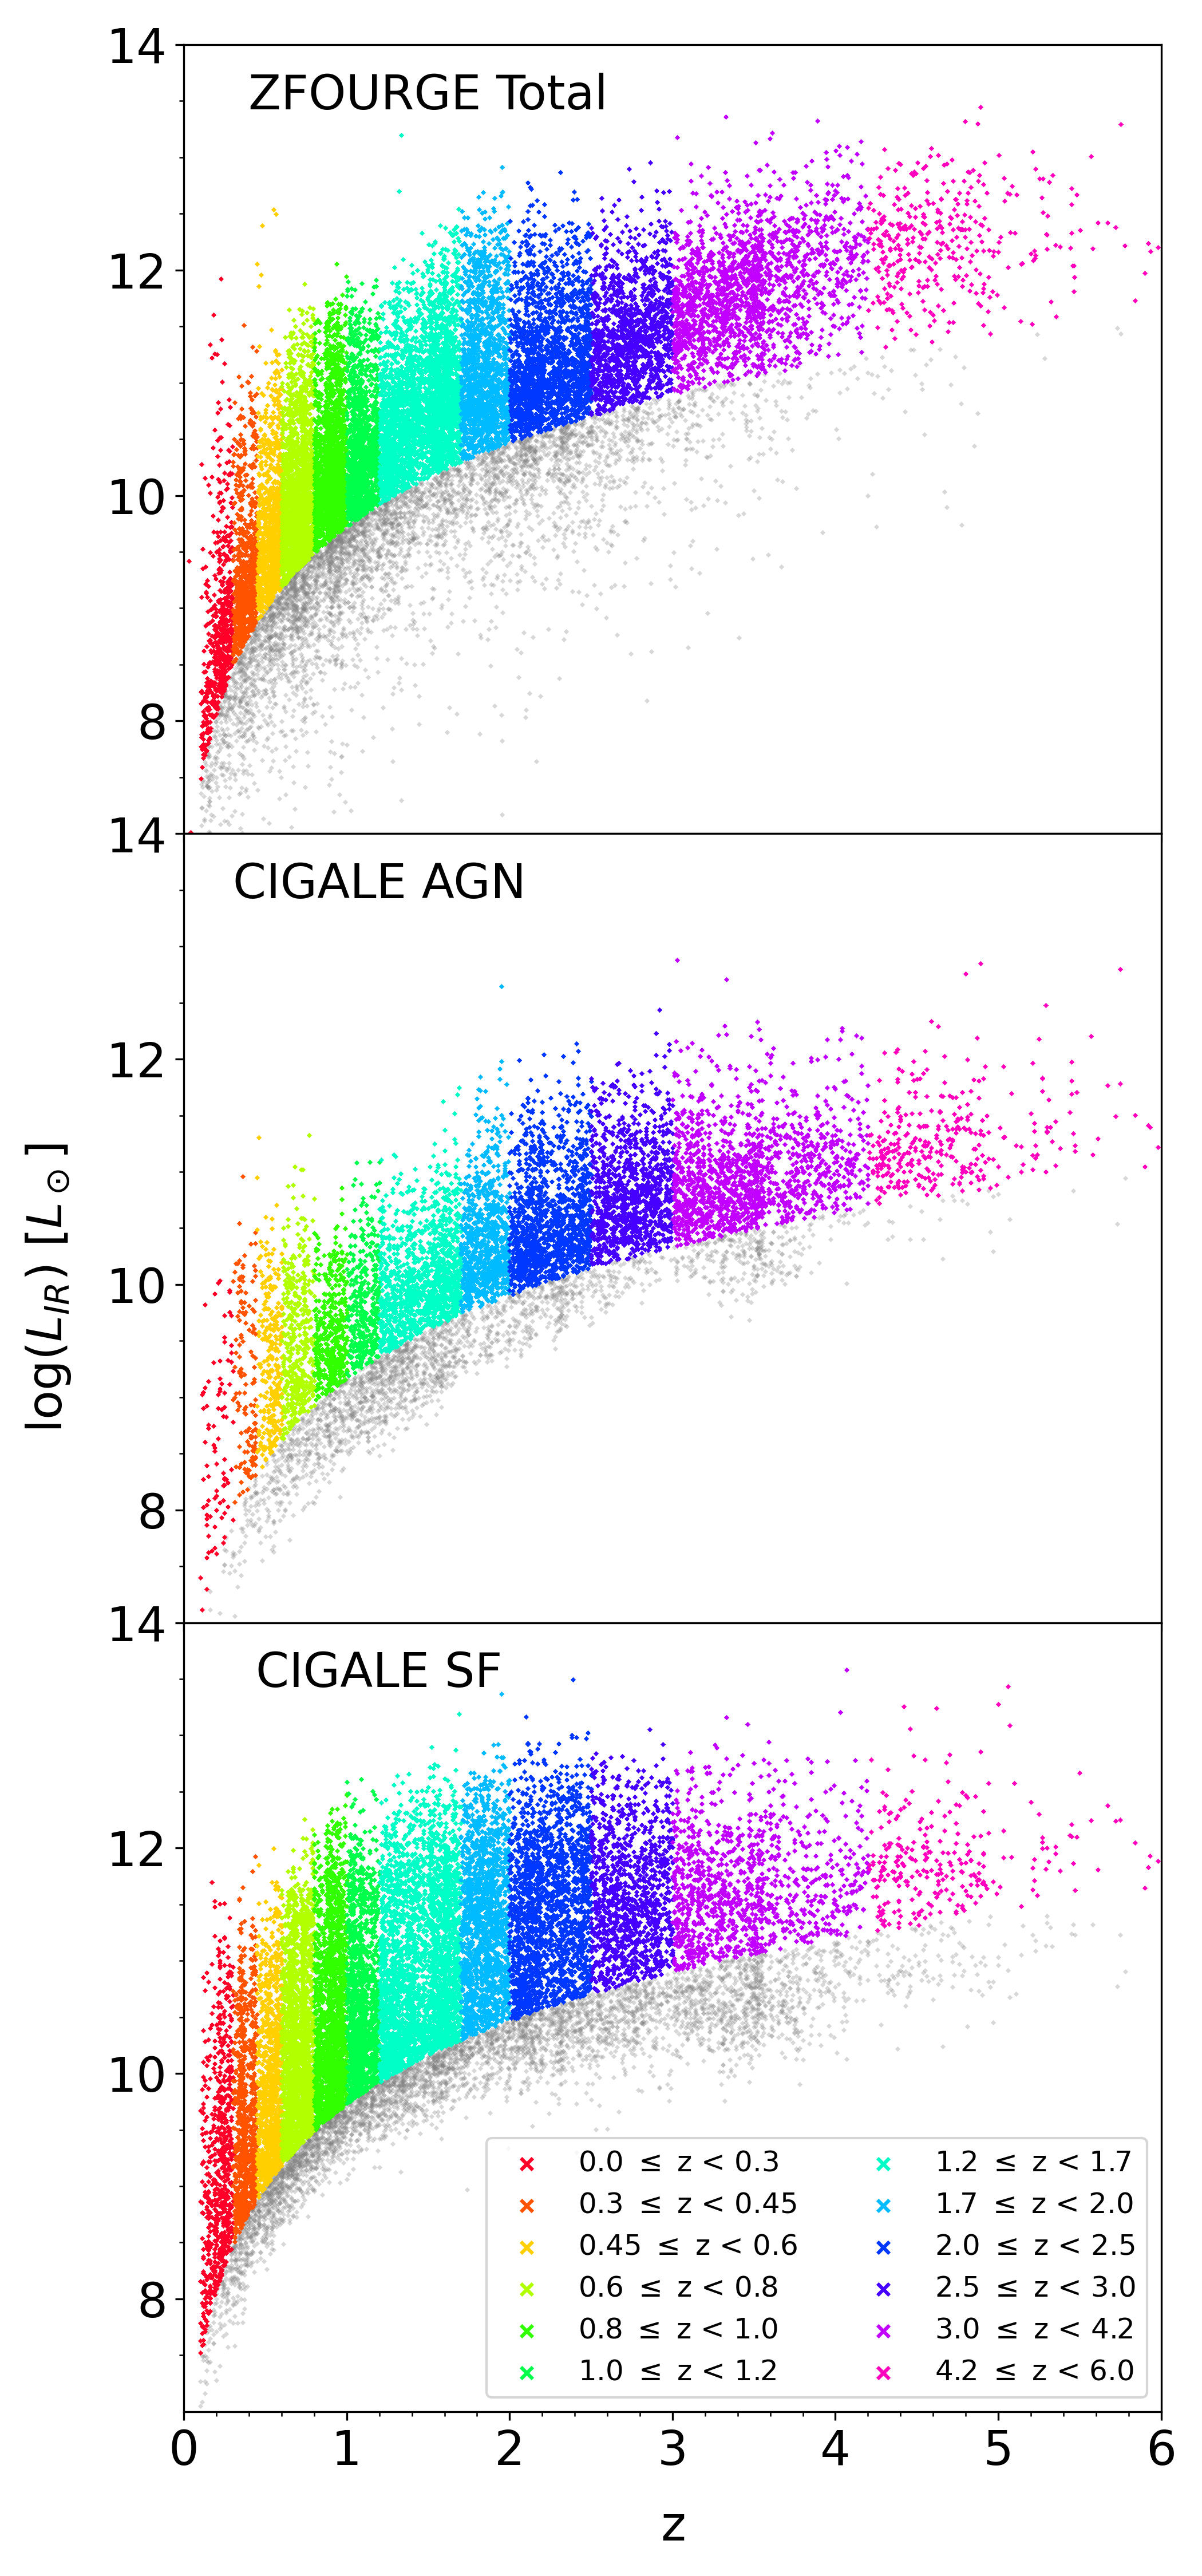
\includegraphics[width=0.48\textwidth]{Figures/LIR vs Z.png}
    \caption{Luminosity-redshift distributions of (top) the ZFOURGE bolometric $8-1000\mu m$ luminosity, (middle) the CIGALE AGN luminosity, and (bottom) the CIGALE SF luminosity. Sources are coloured by redshift bin and are removed (coloured grey) based on the 80\% completeness cut of the bolometric flux for each component respectively.}
    \label{Fig: ZF Lum vs z}
\end{figure}

The 24$\mu$m flux is usually a good proxy for the bolometric flux \citep{rodighiero_mid-_2010}. However, when the 24$\mu$m flux limit is used with the ZFOURGE bolometric luminosity, the limit varies with redshift, possibly due to spectral features shifting in and out of the template fitting process. Instead, we calculate the bolometric flux from the bolometric luminosity and take the 80\% completeness as the flux limit. We calculate the ZFOURGE bolometric flux limit to be $3.882\times10^{-18}$ $W/m^2$. The ZFOURGE star-forming and quiescent dominated sources have very similar flux limits. \textcolor{red}{The CIGALE total and star-forming sources have a flux limit of $5.232\times10^{-18}$ $W/m^2$. The CIGALE AGN flux also varies with redshift, so we calculate the 80\% completeness for each redshift bin individually. Additionally, luminosity completeness limits for ZFOURGE and CIGALE are calculated for each redshift bin. These limits represent the minimum luminosity a galaxy must have to be detectable throughout the entire redshift bin.}